\section{Thử nghiệm và đánh giá}

\subsection{Thiết lập đánh giá}

Toàn bộ thực nghiệm chính được chạy trên workflow \texttt{reproduction/src/run\_full\_demo.py} và các script liên quan. Bộ dữ liệu được tách train/test theo tỉ lệ 80/20, sau đó ba mô hình DT, RF và DT-CTS được huấn luyện trên cùng một tập train để đảm bảo so sánh công bằng. Nhóm đánh giá theo hai hướng:
\begin{itemize}
\item \textbf{Chất lượng phân loại:} accuracy, precision, recall, F1.
\item \textbf{Hiệu quả triển khai và giảm thiểu:} threshold count, latency/FPR/FNR, attack bytes reaching victim, benign bytes preserved và false block events.
\end{itemize}

\subsection{Kết quả phân loại}

\begin{table}
\caption{So sánh kết quả phân loại của ba mô hình trong reproduction chính.}
\label{tab:classification-main}
\centering
\begin{tabular}{lcc}
\toprule
\textbf{Mô hình} & \textbf{Accuracy} & \textbf{F1} \\
\midrule
DT & 0.9901 & 0.9620 \\
RF & 0.9821 & 0.9327 \\
DT-CTS & 0.9800 & 0.9249 \\
\bottomrule
\end{tabular}
\end{table}

Kết quả reproduction chính cho thấy:
\begin{itemize}
\item DT đạt accuracy 0.9901 và F1 0.9620.
\item RF đạt accuracy 0.9821 và F1 0.9327.
\item DT-CTS đạt accuracy 0.9800 và F1 0.9249.
\end{itemize}

Nếu chỉ nhìn riêng F1 thì DT đang là mô hình tốt nhất trong lần chạy hiện tại. Tuy nhiên, điều đáng quan tâm hơn với mục tiêu của SISTAR là DT-CTS vẫn giữ chất lượng ở mức cạnh tranh trong khi được thiết kế để giảm số threshold. Đây mới là điểm quan trọng khi xét tới khả năng triển khai trên programmable switch, nơi chi phí bảng match và số điều kiện so sánh không thể bỏ qua.

\begin{figure}
\centering
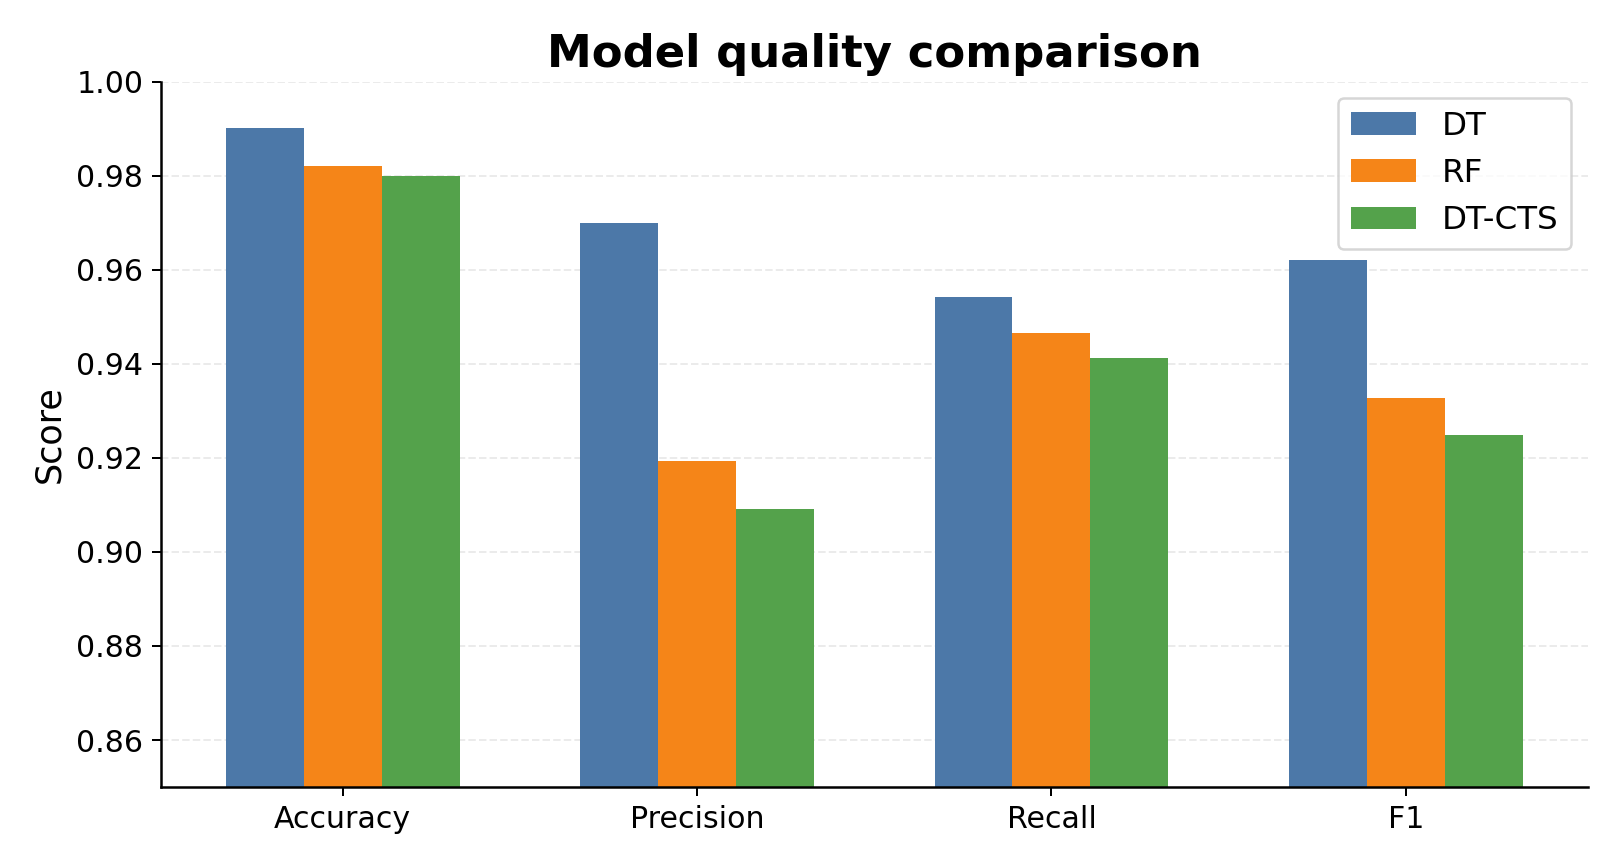
\includegraphics[width=0.78\textwidth]{figures/classification_metric_suite.png}
\caption{So sánh chất lượng phân loại của DT, RF và DT-CTS. DT-CTS thấp hơn nhẹ về F1, nhưng vẫn giữ khoảng cách nhỏ so với hai baseline trong khi hướng đến khả năng triển khai tốt hơn.}
\label{fig:classification-suite}
\end{figure}

\subsection{Hiệu quả theo số lượng threshold}

\begin{table}
\caption{So sánh footprint theo threshold giữa các mô hình chính.}
\label{tab:threshold-main}
\centering
\begin{tabular}{lp{2.1cm}p{4.7cm}}
\toprule
\textbf{Mô hình} & \textbf{Total thresholds} & \textbf{Nhận xét} \\
\midrule
DT & 36 & Baseline dễ hiểu nhưng còn khá nặng \\
RF & rất lớn & Khó phù hợp với data plane \\
DT-CTS & 14 & Giảm 61.11\% so với DT, phù hợp hơn cho switch \\
\bottomrule
\end{tabular}
\end{table}

Trong reproduction chính, DT dùng 36 threshold trong khi DT-CTS chỉ dùng 14 threshold, tương đương mức giảm khoảng 61.11\%. Ở benchmark paper-style với 3, 5 và 7 feature, cấu hình DT-CTS tốt nhất đạt F1 0.9614 với 14 threshold, và vẫn giảm 58.82\% số threshold so với DT cùng cấu hình. Kết quả này cho thấy DT-CTS không nhất thiết vượt lên hoàn toàn về quality, nhưng lại có ưu thế rõ hơn ở trade-off giữa chất lượng và khả năng triển khai.

\begin{figure}
\centering
\begin{subfigure}[t]{0.48\textwidth}
    \centering
    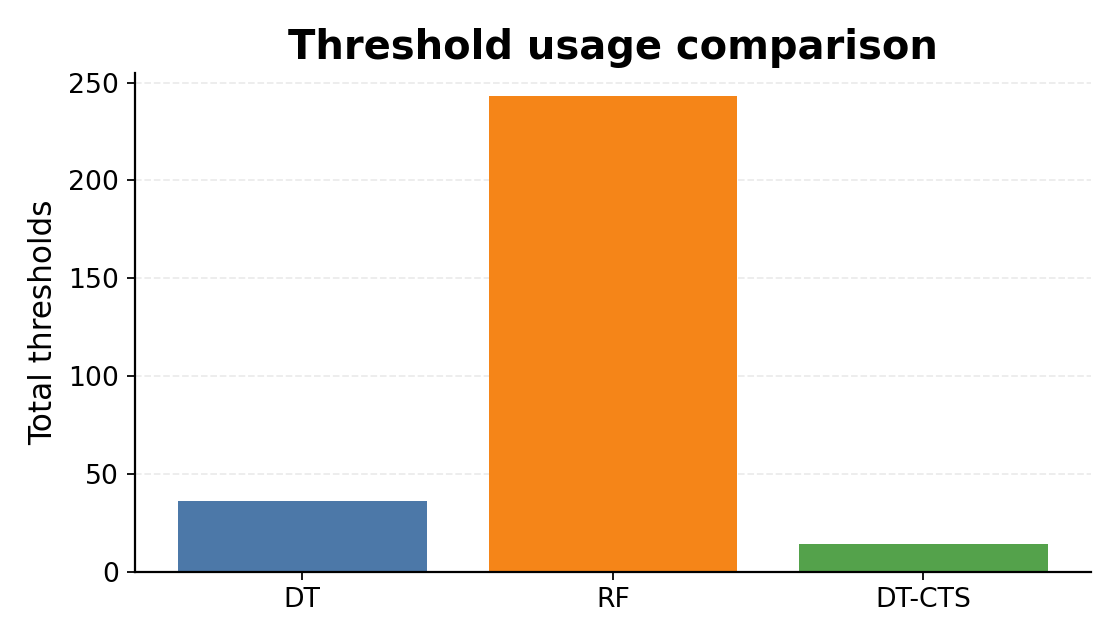
\includegraphics[width=\textwidth]{figures/threshold_usage.png}
    \caption{Threshold usage trong reproduction chính.}
    \label{fig:threshold-usage}
\end{subfigure}\hfill
\begin{subfigure}[t]{0.48\textwidth}
    \centering
    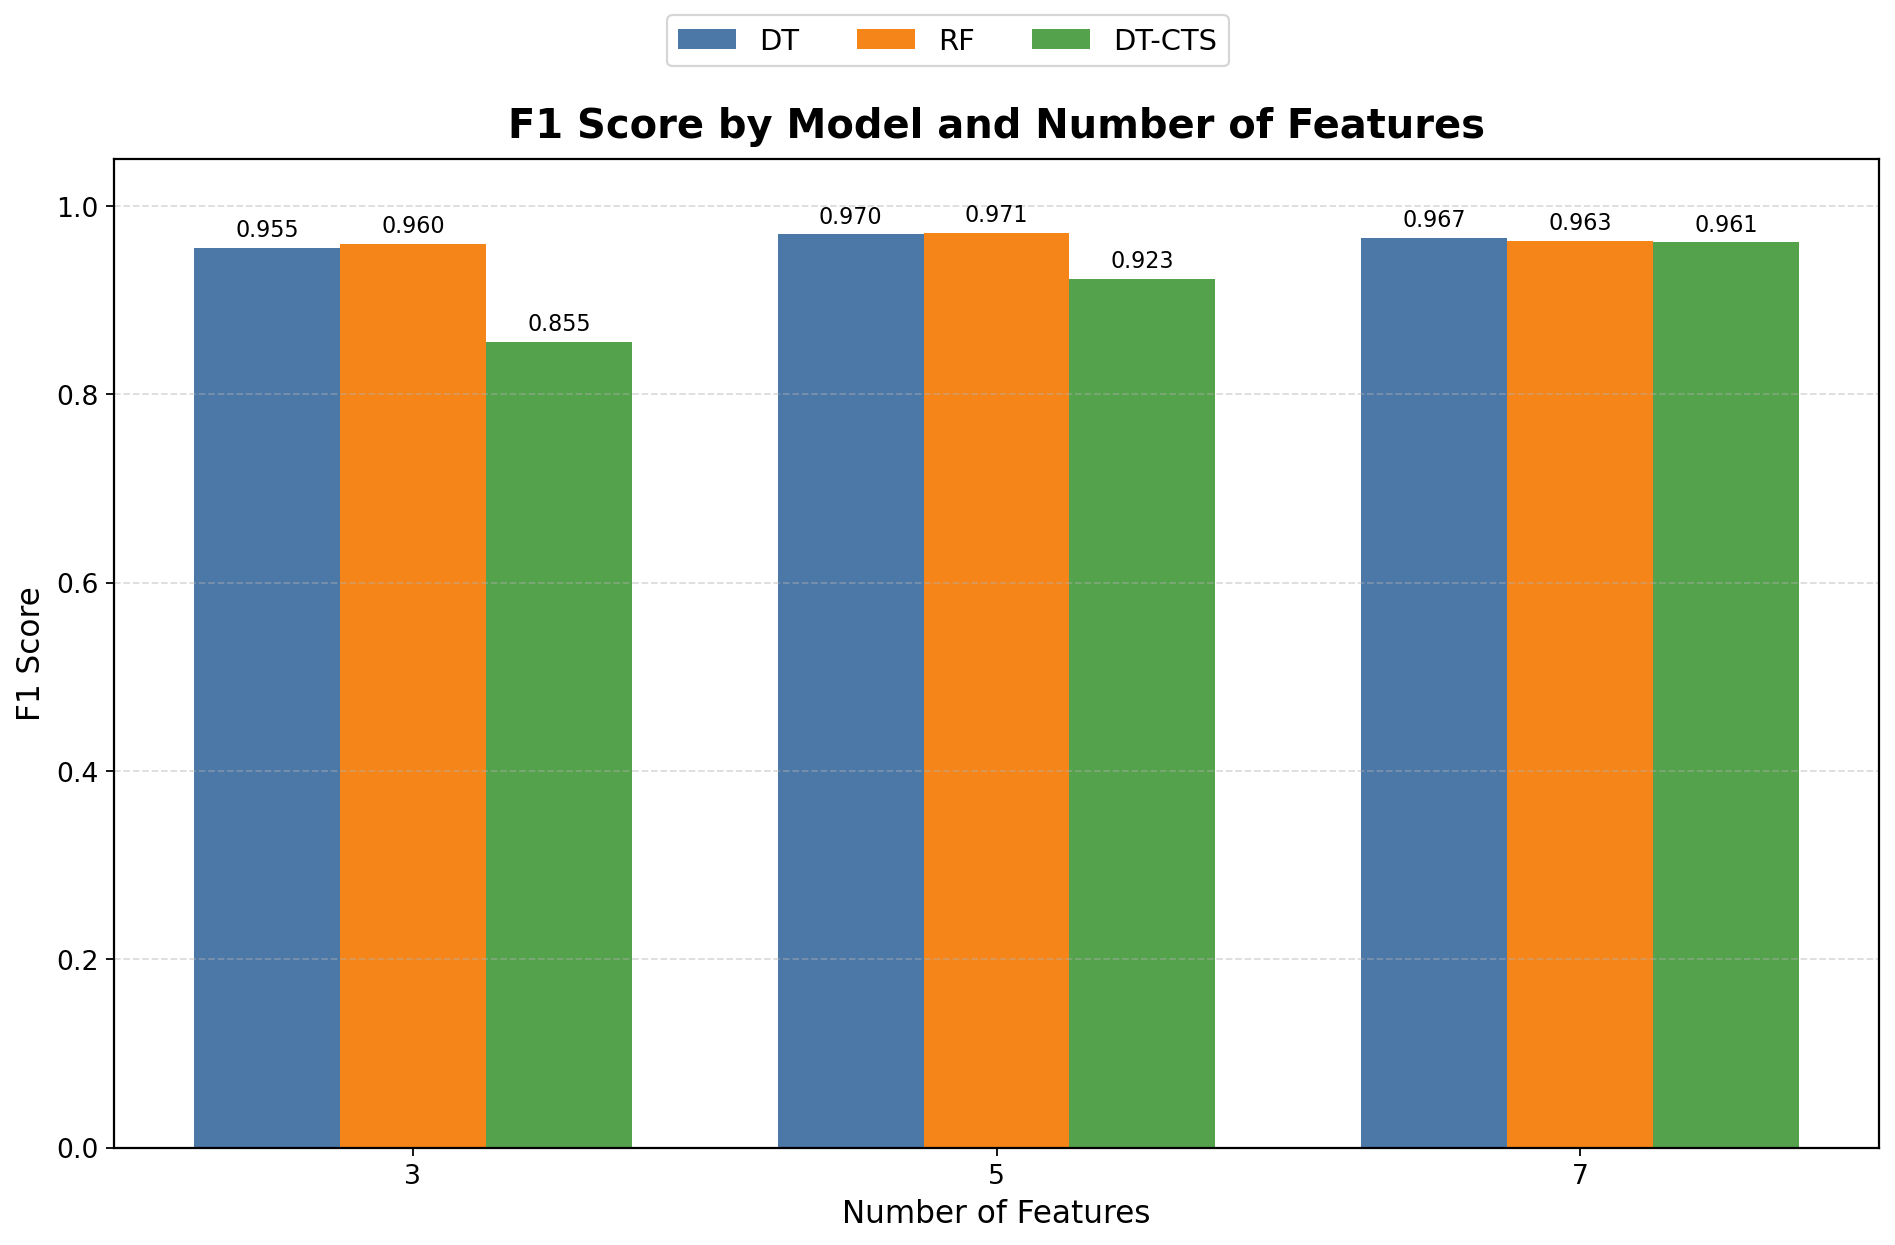
\includegraphics[width=\textwidth]{figures/benchmark_f1_scores.png}
    \caption{F1 trong benchmark paper-style với 3/5/7 feature.}
    \label{fig:benchmark-f1}
\end{subfigure}
\caption{So sánh trade-off giữa chất lượng và footprint. DT-CTS duy trì chất lượng đủ tốt trong khi giảm đáng kể số threshold.}
\label{fig:threshold-benchmark-pair}
\end{figure}

\subsection{Đánh giá cơ chế pushback mới}

\begin{table}
\caption{So sánh ba policy pushback trong thí nghiệm cải tiến.}
\label{tab:pushback-compare}
\centering
\begin{tabular}{lrrc}
\toprule
\textbf{Policy} & \textbf{Attack bytes} & \textbf{Benign bytes} & \textbf{False blocks} \\
\midrule
No pushback & 5{,}876{,}251 & 2{,}196{,}901{,}718 & 0 \\
Immediate pushback & 0 & 1{,}760{,}928{,}313 & 11 \\
Hierarchical pushback & 4{,}591 & 2{,}052{,}047{,}683 & 0 \\
\bottomrule
\end{tabular}
\end{table}

Trong phần giảm thiểu, project so sánh ba policy:
\begin{enumerate}
\item \texttt{no\_pushback}: không giảm thiểu upstream.
\item \texttt{immediate\_pushback}: block ngay sau một lần phát hiện malicious.
\item \texttt{hierarchical\_confidence\_pushback}: policy cải tiến của nhóm.
\end{enumerate}

Kết quả nổi bật như sau:
\begin{itemize}
\item \texttt{no\_pushback}: 5{,}876{,}251 attack bytes tới victim.
\item \texttt{immediate\_pushback}: attack bytes về 0 nhưng có 11 false block events.
\item \texttt{hierarchical\_confidence\_pushback}: chỉ còn 4{,}591 attack bytes tới victim và 0 false block events.
\end{itemize}

So với baseline không pushback, policy mới giảm khoảng 99.92\% attack bytes. Đồng thời, nó vẫn giữ được 2{,}052{,}047{,}683 benign bytes tới victim, cao hơn rõ rệt so với immediate pushback. Điều đó cho thấy phần cải tiến của project có giá trị thực tế: thay vì cố triệt tiêu attack bằng mọi giá, nó ưu tiên một điểm cân bằng tốt hơn giữa phòng thủ và tính sẵn sàng của traffic hợp lệ.

\begin{figure}
\centering
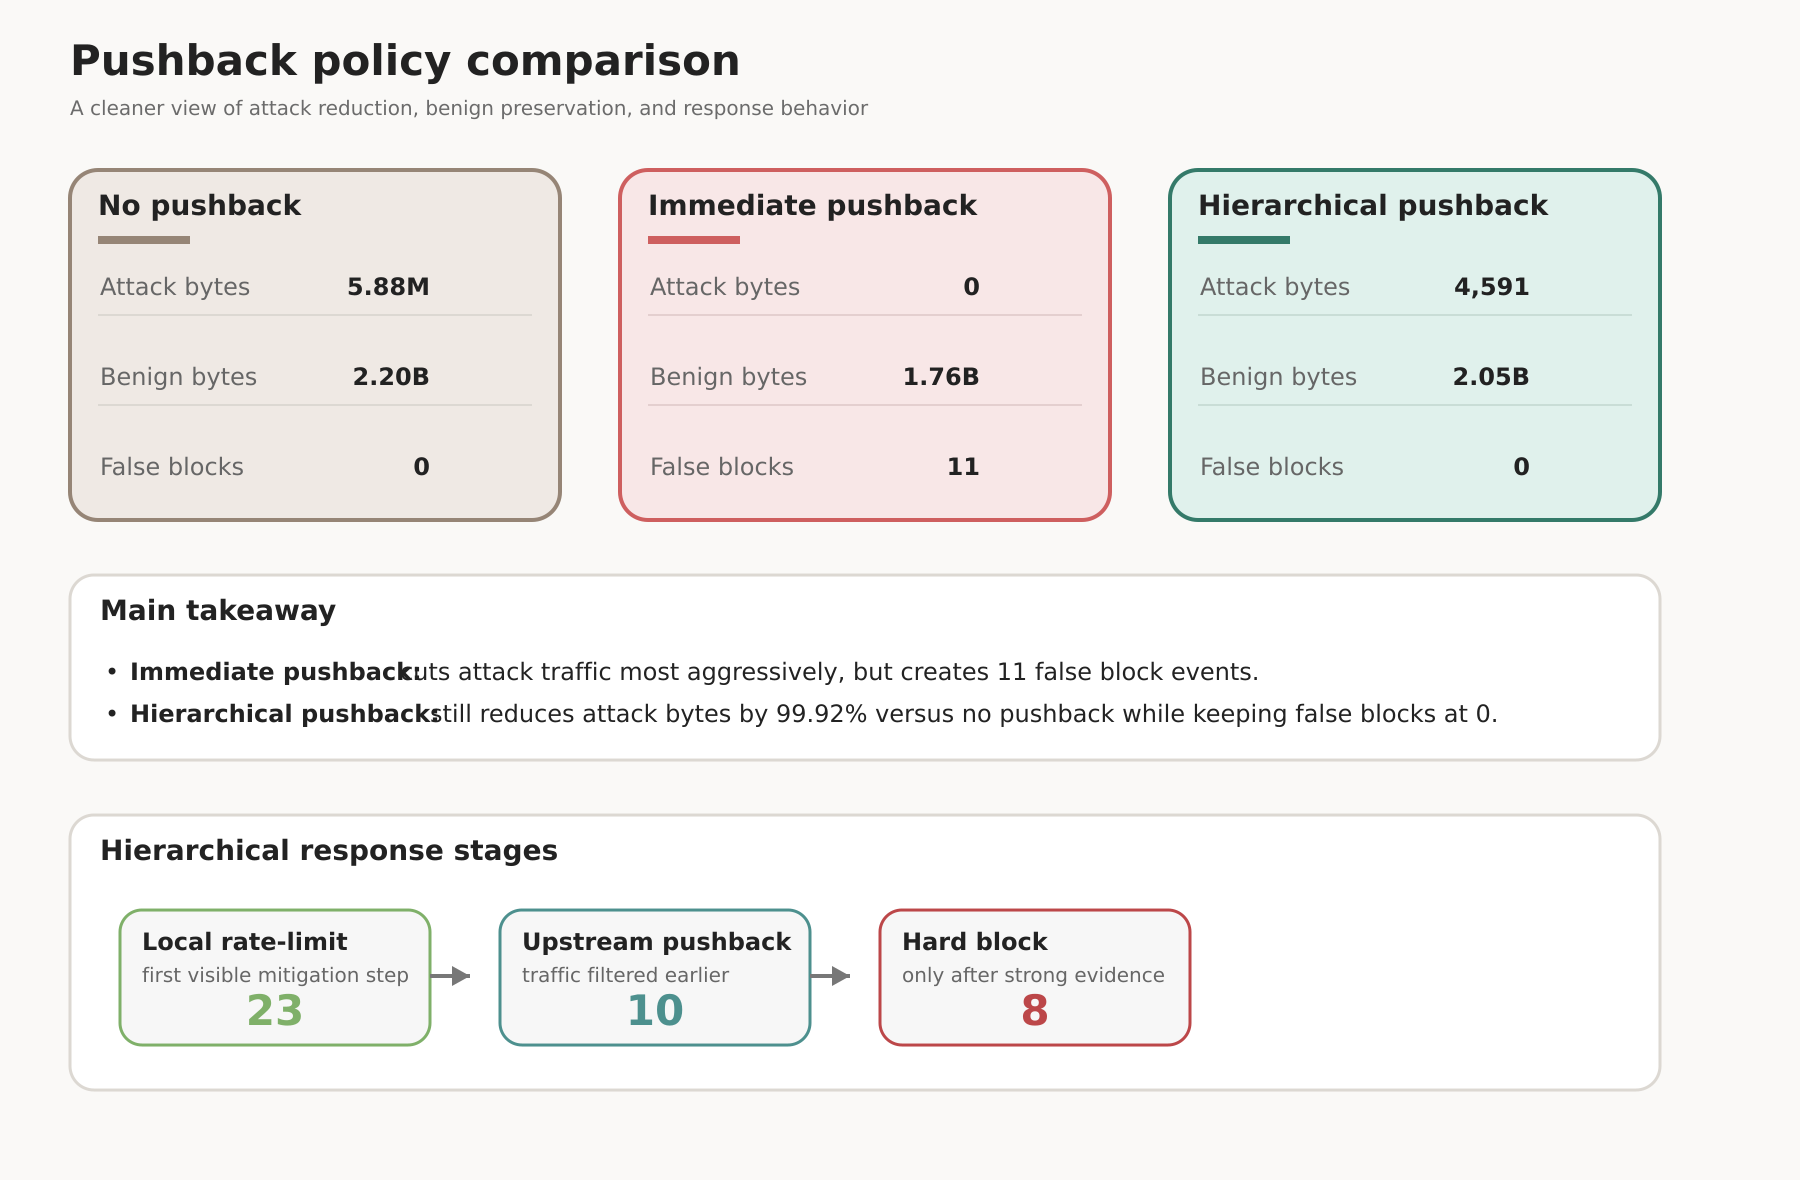
\includegraphics[width=0.95\textwidth]{figures/pushback_clean_summary.png}
\caption{Tóm tắt trực quan kết quả của ba policy pushback. Hình này chỉ giữ lại các thông tin quan trọng nhất: lượng attack traffic còn tới victim, lượng benign traffic được giữ lại, số lần false block và số lần leo thang ở policy cải tiến.}
\label{fig:pushback-clean-summary}
\end{figure}

\subsection{Phân tích hành vi leo thang}

Một điểm đáng chú ý là policy mới thực sự sử dụng các mức trung gian chứ không nhảy thẳng lên hard block. Trong lần chạy hiện tại, hệ thống ghi nhận 23 local rate-limit events, 10 upstream pushback events và 8 hard block events. Điều này cho thấy suspicion score thực sự đóng vai trò như một bộ nhớ trạng thái, giúp hệ thống đánh giá lại source qua nhiều window thay vì ra quyết định chỉ từ một dự đoán duy nhất.

\subsection{Thảo luận}

Từ các kết quả trên có thể rút ra ba nhận xét. Thứ nhất, DT-CTS là lựa chọn hợp lý khi mục tiêu bao gồm cả triển khai data plane chứ không chỉ dừng ở classification quality. Thứ hai, immediate pushback rất mạnh trong việc triệt tiêu attack nhưng lại quá nhạy với false positive. Thứ ba, hierarchical confidence-aware pushback giải quyết bài toán ở cấp hệ thống tốt hơn vì nó cho phép phản ứng theo mức, gần với cách một hệ thống thực tế nên vận hành.

Tất nhiên, báo cáo vẫn còn một số giới hạn. Các kết quả pushback hiện mới được đo trong mô phỏng flow-level, chưa phải trên mạng thật hoặc ASIC thật. Ngoài ra, threshold count cũng chỉ là chỉ báo gián tiếp cho footprint phần cứng. Dù vậy, các kết quả hiện tại vẫn đủ để cho thấy hướng cải tiến của nhóm là hợp lý và có ý nghĩa hơn một thay đổi nhỏ ở ngưỡng block.
